        \clearpage
        \begin{figure*}[ht]
            \pdfbookmark[2]{ID 04}{figure_id_04}
        	\centering
            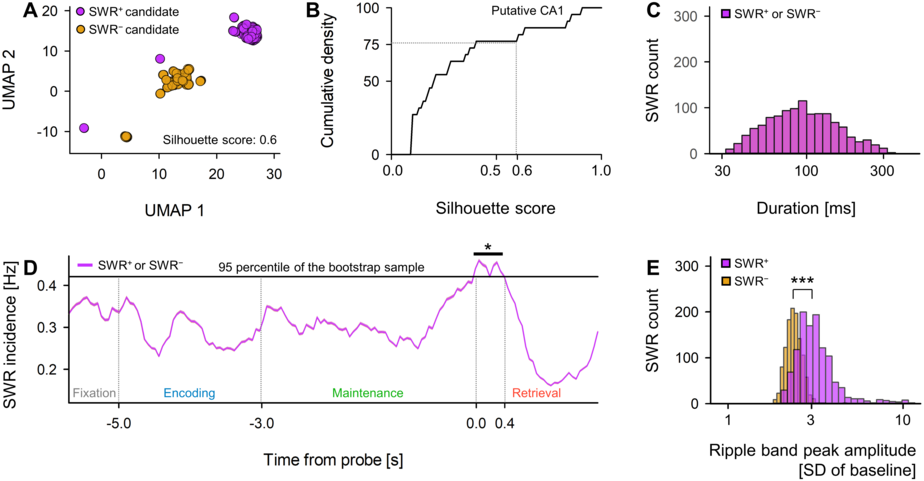
\includegraphics[width=1\textwidth]{./media/figures/.png/Figure_ID_04.png}
        	\caption{\textbf{
SWR detection in putative CA1 regions
}
\smallskip
\\
\textbf{\textit{A.}} Two-dimensional UMAP (uniform manifold approximation and projection)\cite{mcinnes_umap_2018} representation of unit activities during SWR$^+$ candidates (\textit{purple}; potential SWR events) and SWR$^-$ candidates (\textit{yellow}; controls for SWR$^+$ candidates). \textbf{\textit{B.}}  Cumulative density plot illustrating silhouette scores for different hippocampal regions (refer to Table 2). Regions with silhouette scores exceeding 0.60 ($75^{th}$ percentile) are considered as putative CA1 regions. Within these regions, SWR$^+$ and SWR$^-$ candidates are identified and categorized as SWR$^+$ (\textit{n} = 1,170) and SWR$^-$ (\textit{n} = 1,170), respectively. \textbf{\textit{C.}}  Overlapping duration distributions [ms] for SWR$^+$ (\textit{purple}; 93.0 [65.4], median [IQR]) and SWR$^-$ (\textit{yellow}; 93.0 [65.4], median [IQR]). The identical overlap results from their definition criteria. \textbf{\textit{D.}}  Depiction of ripple incidence [Hz] for both SWR$^+$ (\textit{purple}) and SWR$^-$ (\textit{yellow}) relative to time from the probe, represented as mean \textpm 95\% confidence interval. However, the 95\% confidence interval might not be readily discernible due to its narrow range. Note the significant elevation in SWR incidence between 0--400 ms post-probe, surpassing the 95th percentile of bootstrap samples (0.421 [Hz], *\textit{p} $<$ 0.05). \textbf{\textit{E.}}  Histogram showcasing ripple band peak amplitude distributions for SWR$^-$ (\textit{yellow}; 2.37 [0.33], median [IQR]) versus SWR$^+$ (\textit{purple}; 3.05 [0.85], median [IQR]). A notable difference is present between the two, confirmed with ***\textit{p} $<$ 0.001 using the Brunner--Munzel test.
}
% width=1\textwidth
        	\label{fig:04}
        \end{figure*}
